\documentclass[oneside]{ntuthesis}

\usepackage{times}
\usepackage{verbatim}
\usepackage{color}
\usepackage{url}
\usepackage{graphicx}
\usepackage{array}
\usepackage{pdfpages} % include outside .pdf
\usepackage{wallpaper} % watermark

% Format the refs
\usepackage[sort,comma]{natbib}
\usepackage[hidelinks]{hyperref}

% For the tree
\usepackage{tikz}
\usepackage{tikz-qtree}

% For barchart
\usepackage{pgfplots}

% Using the tex-text mapping for ligatures etc.
\defaultfontfeatures{Mapping=tex-text}

% Set the default fonts
\setmainfont{Times New Roman}
\setCJKmainfont{標楷體}

% Your information goes here
% author: Tz-Huan Huang [http://www.csie.ntu.edu.tw/~tzhuan]

% ----------------------------------------------------------------------------
% "THE CHOCOLATE-WARE LICENSE":
% Tz-Huan Huang wrote this file. As long as you retain this notice you
% can do whatever you want with this stuff. If we meet some day, and you think
% this stuff is worth it, you can buy me a chocolate in return Tz-Huan Huang
% ----------------------------------------------------------------------------

% Syntax: \var{English}{Chinese}
\university{National Taiwan University}{國立臺灣大學}
\college{College of Electrical Engineering and Computer Science}{電機資訊學院}
\institute{Department of Computer Science and Information Engineering}{資訊工程學系}
\title{Master's Thesis in Computer Science}{資訊系中碩士生學位論文之研究}
\author{Siao-Ming Wang}{王小明}
\studentid{R00000000}
\advisor{Da-Ming Wang, Ph.D.}{王大明\ 博士}
\defenseyear{2015}{104}
\defensemonth{July}{7}
\defenseday{31}


\begin{document}

% 臺大論文浮水印
\input{watermark.tex}

\hypersetup{pageanchor=false}

\frontmatter
\pagenumbering{gobble}
\makecover

\clearpages
\setcounter{page}{1}
\hypersetup{pageanchor=true}
\pagenumbering{roman}
\phantomsection

\makecertification
% or include scanned pdf
%\addcontentsline{toc}{chapter}{口試委員會審定書}
%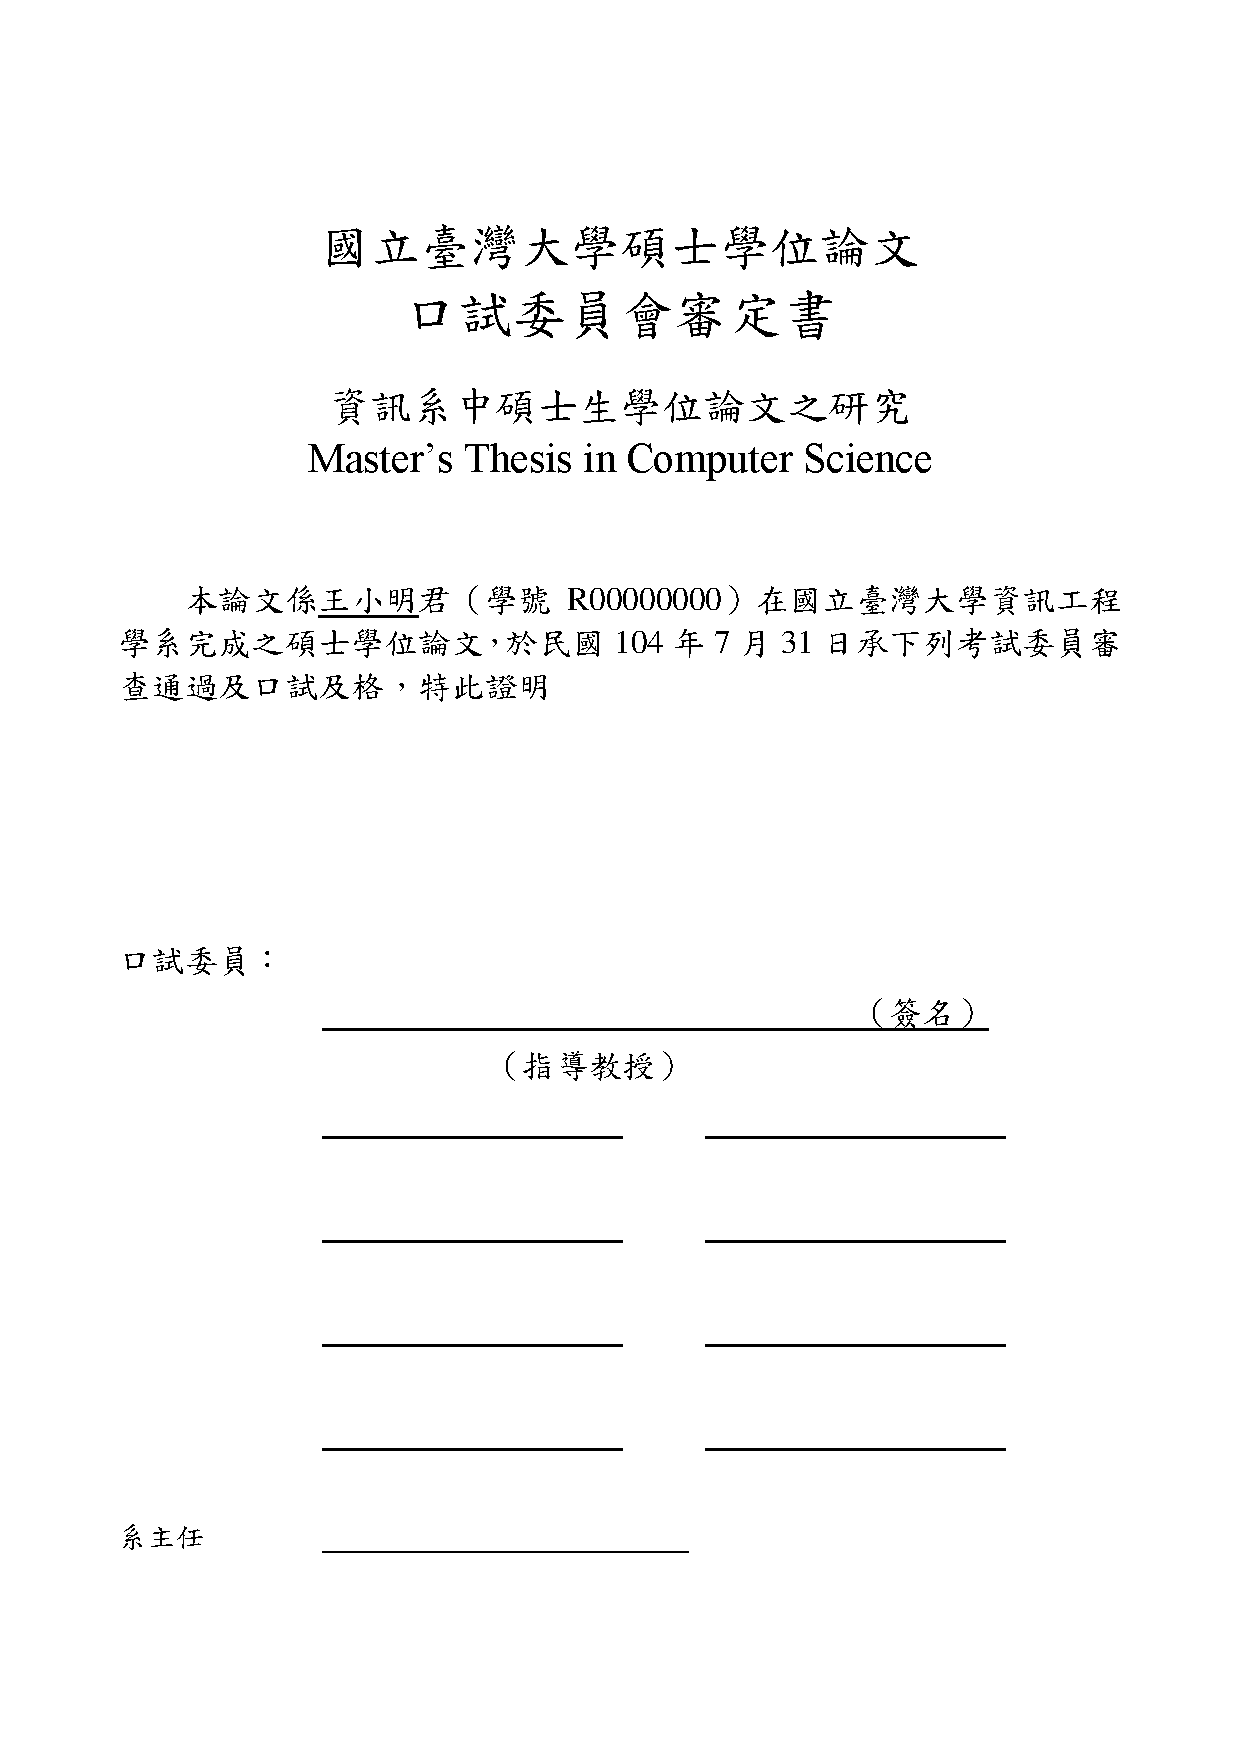
\includepdf[pages={1}]{pdfs/cert.pdf}

\begin{acknowledgementszh}
假的,什麼都是假的,畢業才是真的

\end{acknowledgementszh}

% 自行決定是否需英文摘要
% \begin{acknowledgementsen}
% This is English line spacing test. You should see double spacing text.
% This is English line spacing test. You should see double spacing text.
% This is English line spacing test. You should see double spacing text.
% This is English line spacing test. You should see double spacing text.
% This is English line spacing test. You should see double spacing text.
% This is English line spacing test. You should see double spacing text.
% This is English line spacing test. You should see double spacing text.
% This is English line spacing test. You should see double spacing text.

% I'm glad to thank\ldots 
% \end{acknowledgementsen}

\begin{abstractzh}
本論文提出了一影像中使用者感興趣區域 (region of interest)
偵測之資料集 (benchmark)。
使用者感興趣區域偵測在許多應用中極為有用,
過去雖然有許多使用者感興趣區域之自動偵測演算法被提出,
然而由於缺乏公開資料集,
這些方法往往只測試了各自的小量資料而難以互相比較。
從其它領域可以發現,
基於公開資料集的可重製實驗與該領域突飛猛進密切相關,
因此本論文填補了此領域之不足,
我們提出名為「Photoshoot」的遊戲來蒐集人們對於感興趣區域的標記,
並以這些標記來建立資料集。
透過這個遊戲,我們已蒐集大量使用者對於感興趣區域的標記,
並結合這些資料成為使用者感興趣區域模型。
我們利用這些模型來量化評估五個使用者感興趣區域偵測演算法,
此資料集也可更進一步作為基於學習理論演算法的測試資料,
因此使基於學習理論的偵測演算法成為可能。
\end{abstractzh}

\begin{abstracten}
This thesis presents a benchmark for region of interest (ROI)
detection. ROI detection has many useful applications and many
algorithms have been proposed to automatically detect ROIs.
Unfortunately, due to the lack of benchmarks, these methods were
often tested on small data sets that are not available to others,
making fair comparisons of these methods difficult. Examples from
many fields have shown that repeatable experiments using published
benchmarks are crucial to the fast advancement of the fields. To
fill the gap, this thesis presents our design for a collaborative
game, called Photoshoot, to collect human ROI annotations for
constructing an ROI benchmark. With this game, we have gathered a
large number of annotations and fused them into aggregated ROI
models. We use these models to evaluate five ROI detection
algorithms quantitatively. Furthermore, by using the benchmark as
training data, learning-based ROI detection algorithms become
viable.
\end{abstracten}

\begin{comment}
\category{I2.10}{Computing Methodologies}{Artificial Intelligence --
Vision and Scene Understanding} \category{H5.3}{Information
Systems}{Information Interfaces and Presentation (HCI) -- Web-based
Interaction.}

\terms{Design, Human factors, Performance.}

\keywords{Region of interest, Visual attention model, Web-based
games, Benchmarks.}
\end{comment}


% Table of Content
\clearpages
\tableofcontents
% List of Figures
\clearpages
\listoffigures
% List of Tables
\clearpages
\listoftables

\mainmatter

% Your thesis goes here
\chapter{Introduction}
\label{c:intro}

Recently a cat appears in NTU as shown in Figure~\ref{i:cat}.
This is English line spacing test. You should see double spacing text.
This is English line spacing test. You should see double spacing text.
This is English line spacing test. You should see double spacing text.

%i:cat
\begin{figure}[!htbp]
\centering
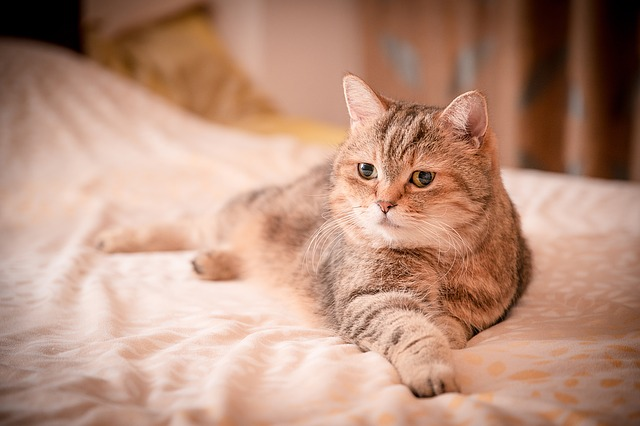
\includegraphics{images/cat}
\caption{A cat.}
\label{i:cat}
\end{figure}


As \cite{o2014cats} pointed out, there were many videos~\citep{o2014cats}.

\chapter{文獻探討}

\section{好想畢業}


測試文字我想畢業測試文字我想畢業測試文字我想畢業測試文字我想畢業測試文字我想畢業測試文字我想畢業測試文字我想畢業測試文字我想畢業測試文字我想畢業測試文字我想畢業測試文字我想畢業測試文字我想畢業測試文字我想畢業測試文字我想畢業測試文字我想畢業測試文字我想畢業測試文字我想畢業測試文字我想畢業測試文字我想畢業測試文字我想畢業測試文字我想畢業測試文字我想畢業測試文字我想畢業測試文字我想畢業測試文字我想畢業測試文字我想畢業測試文字我想畢業測試文字我想畢業測試文字我想畢業測試文字我想畢業測試文字我想畢業測試文字我想畢業測試文字我想畢業測試文字我想畢業測試文字我想畢業測試文字我想畢業測試文字我想畢業測試文字我想畢業測試文字我想畢業測試文字我想畢業測試文字我想畢業測試文字我想畢業測試文字我想畢業測試文字我想畢業測試文字我想畢業測試文字我想畢業測試文字我想畢業測試文字我想畢業測試文字我想畢業測試文字我想畢業測試文字我想畢業測試文字我想畢業測試文字我想畢業測試文字我想畢業測試文字我想畢業測試文字我想畢業測試文字我想畢業測試文字我想畢業測試文字我想畢業測試文字我想畢業




\chapter{研究方法}
\section{研究設計與流程}
測試文字我想畢業測試文字我想畢業測試文字我想畢業測試文字我想畢業測試文字我想畢業測試文字我想畢業測試文字我想畢業測試文字我想畢業測試文字我想畢業測試文字我想畢業測試文字我想畢業測試文字我想畢業測試文字我想畢業測試文字我想畢業測試文字我想畢業測試文字我想畢業測試文字我想畢業測試文字我想畢業測試文字我想畢業測試文字我想畢業測試文字我想畢業測試文字我想畢業測試文字我想畢業測試文字我想畢業測試文字我想畢業測試文字我想畢業測試文字我想畢業測試文字我想畢業測試文字我想畢業測試文字我想畢業測試文字我想畢業測試文字我想畢業測試文字我想畢業測試文字我想畢業測試文字我想畢業測試文字我想畢業測試文字我想畢業測試文字我想畢業測試文字我想畢業測試文字我想畢業測試文字我想畢業測試文字我想畢業測試文字我想畢業測試文字我想畢業測試文字我想畢業測試文字我想畢業測試文字我想畢業測試文字我想畢業測試文字我想畢業測試文字我想畢業測試文字我想畢業測試文字我想畢業測試文字我想畢業測試文字我想畢業測試文字我想畢業測試文字我想畢業測試文字我想畢業測試文字我想畢業測試文字我想畢業測試文字我想畢業

本研究吉祥物如圖~\ref{i:cat}。
\begin{figure}[!htbp]
\centering
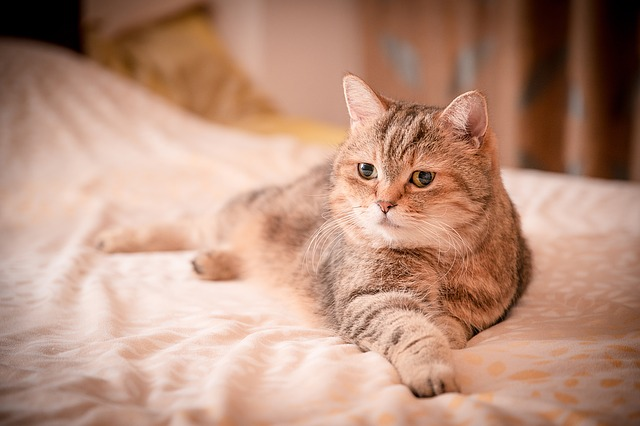
\includegraphics{images/cat}
\caption{A cat.}
\label{i:cat}
\end{figure}


樹範例如~\ref{i:tree}
\begin{figure}[!htbp]
\centering
\tikzset{every tree node/.style={align=center},
    level distance=40pt,
    sibling distance=6pt}
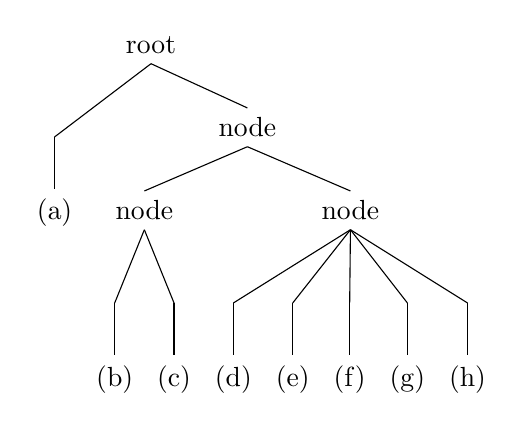
\begin{tikzpicture}
\Tree[.root
       [ (a) ]
       [.node
         [.node
           [ (b) ]
           [ (c) ]
         ]
         [.node
           [ (d) ]
           [ (e) ]
           [ (f) ]
           [ (g) ]
           [ (h) ]
         ]
       ]
     ]

\end{tikzpicture}

\caption{A tree. }
\label{i:tree}
\end{figure}


長條圖範例如~\ref{i:barchart}
\begin{figure}[!htbp]
    \centering
    \vspace{2em}
    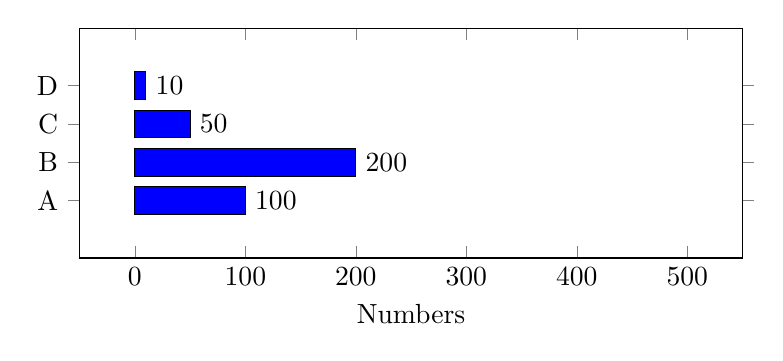
\begin{tikzpicture}
        \begin{axis}[
            enlarge y limits=0.5,
            enlarge x limits=0.1,
            height=4.5cm,
            width=10cm,
            symbolic y coords={A,B,C,D},
            xmin=0,
            xmax=500,
            xbar=1pt,
            xlabel=Numbers,
            nodes near coords={\pgfmathprintnumber[/pgf/number format/assume math mode]{\pgfplotspointmeta}},
            nodes near coords align={horizontal},
            every node near coord/.append style={
                anchor=west}
            ,
            xticklabel style={/pgf/number format/assume math mode},
            yticklabel style={/pgf/number format/assume math mode},
            ytick=data
          ]
            \addplot[xbar,fill=blue] coordinates {
            (100,A)
            (200,B)
            (50,C)
            (10,D)
            };
        \end{axis}
    \end{tikzpicture}
    \caption{A barchart.}
    \label{i:barchart}
\end{figure}



本研究分組如表~\ref{t:group}
\begin{table}[!htbp]
\centering
\caption{實驗分組}
\label{t:group}
\begin{adjustbox}{max width=\textwidth}
\begin{tabular}{@{}ccc@{}}
\toprule
\textbf{\begin{tabular}[c]{@{}c@{}}第一部分題目\\ Q1 Q2 Q3\end{tabular}} & \textbf{\begin{tabular}[c]{@{}c@{}}第二部分題目\\ Q4\end{tabular}} & \textbf{組別} \\ \midrule
abc & abc & 4 \\
abc & abc & 2 \\
abc & abc & 3 \\
abc & abc & 1 \\ \bottomrule
\end{tabular}
\end{adjustbox}
\newline
\small{資料來源:本研究}
\end{table}






    







\chapter{實驗結果}
\label{c:experiment}

\section{描述性統計}
本研究各變數實驗結果之描述性統計(個數、最小值、最大值、平均與標準差)如表~\ref{4-0}。

\begin{table}[htbp]
\centering
\caption{受測者描述性統計}
\label{4-0}
\begin{adjustbox}{max width=0.92\textwidth}
\begin{tabular}{llrrrrr}

\toprule
\multicolumn{2}{l}{\textbf{變數}} & \textbf{個數} & \textbf{最小值} & \textbf{最大值} & \textbf{平均數} & \textbf{標準差} \\ \midrule
\multicolumn{1}{l}{\textbf{背景}} & \textbf{} & \textbf{} & \textbf{} & \textbf{} & \textbf{} & \textbf{} \\

\multicolumn{1}{l}{\textbf{資料}} & \textbf{} & \textbf{} & \textbf{} & \textbf{} & \textbf{} & \textbf{} \\

\multicolumn{1}{l}{\textbf{資料}} & \textbf{} & \textbf{} & \textbf{} & \textbf{} & \textbf{} & \textbf{} \\
\bottomrule
\end{tabular}
\end{adjustbox}
\end{table}


\section{實驗結果分析}

如表~\ref{4-4},以雙獨立樣本t檢定檢驗...

\begin{table}[htbp]
\centering
\caption{測試(N=50)}
\label{4-4}
\begin{adjustbox}{max width=\textwidth}
\begin{tabular}{@{}ccccclrc@{}}
\toprule
 & \multicolumn{2}{c}{測試一} & \multicolumn{2}{c}{測試二} &  &  &  \\ \cmidrule(lr){2-5}
 & 平均 & 標準差 & 平均 & 標準差 & 自由度 & t值 & \textit{p-value} \\ \midrule
Q1 & 3.58 & 1.64 & 3.23 & 1.84 & 48 & -.71 & .47 \\
Q2 & 3.71 & 1.48 & 4.04 & 1.42 & 48 & .80 & .42 \\
Q3 & 5.46 & 2.22 & 6.15 & 1.51 & 40.126 & 1.28 & .20 \\ \bottomrule
\end{tabular}
\end{adjustbox}
\end{table}





如表~\ref{4-9}所示...

\begin{sidewaystable}

\centering
\caption{測試anova(N=50)}
\label{4-9}
\begin{adjustbox}{max width=\textwidth}
\begin{tabular}{@{}crrrrr@{}}

\toprule
\multicolumn{1}{l}{} & \multicolumn{1}{c}{\begin{tabular}[c]{@{}c@{}}G1\\ 測試\\ N=12\\ (M/SD)\end{tabular}} & \multicolumn{1}{c}{\begin{tabular}[c]{@{}c@{}}G2\\ 測試\\ N=12\\ (M/SD)\end{tabular}} & \multicolumn{1}{c}{\begin{tabular}[c]{@{}c@{}}G3\\ 測試\\ N=14\\ (M/SD)\end{tabular}} & \multicolumn{1}{c}{\begin{tabular}[c]{@{}c@{}}G4\\ 測試\\ N=12\\ (M/SD)\end{tabular}} & \multicolumn{1}{c}{\begin{tabular}[c]{@{}c@{}}F\\ (df)\end{tabular}} \\
\midrule
\multicolumn{1}{l}{變數名稱} & \multicolumn{1}{c}{} & \multicolumn{1}{c}{} & \multicolumn{1}{c}{} & \multicolumn{1}{c}{} & \multicolumn{1}{c}{} \\
測試 & (7.25/1.76) & (6.00/1.80) & (6.43/1.91) & (6.42/1.73) & \begin{tabular}[c]{@{}r@{}}1.00\\ (3,46)\end{tabular} \\
測試 & (40.16/12.01) & (40.08/11.13) & (34.35/10.93) & (36.33/7.66) & \begin{tabular}[c]{@{}r@{}}.95\\ (3,46)\end{tabular} \\
測試 & (68.83/14.04) & (68.83/23.37) & (79.21/22.73) & (81.75/30.13) & \begin{tabular}[c]{@{}r@{}}1.05\\ (3,46)\end{tabular} \\
測試 & (39.25/74.65) & (10.66/91.36) & (30.71/38.42) & (18.00/90.86) & \begin{tabular}[c]{@{}r@{}}.19\\ (3,46)\end{tabular} \\
測試 & (1.37/.42) & 高(1.58/.82) & (1.11/.62) & 低(.80/.63) & \begin{tabular}[c]{@{}r@{}}3.33*\\ (3,46)\end{tabular} \\
測試 & (04.66/12.66) & (39.83/11.26) & (71.92/29.64) & (39.50/19.43) & \begin{tabular}[c]{@{}r@{}}.71\\ (3,46)\end{tabular} \\
測試 & (4.84/1.21) & (5.14/1.41) & (4.59/1.12) & (4.78/1.45) & \begin{tabular}[c]{@{}r@{}}.40\\ (3,46)\end{tabular} \\
測試 & (10.45/34.43) & (05.12/41.36) & (87.46/34.60) & (95.20/30.74) & \begin{tabular}[c]{@{}r@{}}1.08\\ (3,46)\end{tabular} \\
\bottomrule
\end{tabular}
\end{adjustbox}

\end{sidewaystable}





\chapter{Conclusions}
\label{c:conclusion}


\appendix

\backmatter

\clearpages
\phantomsection
\addcontentsline{toc}{chapter}{\bibname}
\bibliographystyle{apa}

% Your bibliography goes here
\bibliography{thesis}

\end{document}
